\documentclass[11pt,a4paper]{article}
\usepackage[T1]{fontenc}
\usepackage[utf8]{inputenc}
\usepackage{charter}
\usepackage[scaled=0.9]{helvet}
\usepackage[a4paper,margin=2.2cm]{geometry}
\usepackage{graphicx,booktabs,array,longtable,enumitem,microtype}
\usepackage[dvipsnames]{xcolor}
\usepackage[font=small,labelfont=bf,skip=4pt]{caption}
\usepackage{titlesec}
\usepackage[colorlinks=true,linkcolor=MidnightBlue,urlcolor=MidnightBlue]{hyperref}
\definecolor{ink}{HTML}{1A1A1A}\definecolor{accent}{HTML}{2A78D6}
\titleformat{\section}{\sffamily\Large\bfseries\color{ink}}{}{0pt}{}
\titleformat{\subsection}{\sffamily\large\bfseries\color{ink}}{}{0pt}{}
\titlespacing*{\section}{0pt}{14pt}{6pt}
\titlespacing*{\subsection}{0pt}{10pt}{4pt}
\setcounter{secnumdepth}{0}
\renewcommand{\thetable}{S\arabic{table}}
\renewcommand{\thefigure}{S\arabic{figure}}
\setlist[itemize]{leftmargin=1.3em,itemsep=3pt,topsep=4pt}
\setlength{\parskip}{5pt}\setlength{\parindent}{0pt}
\renewcommand{\arraystretch}{1.15}
\begin{document}

{\sffamily\bfseries\color{accent}\large Supplementary Material}\\[4pt]
{\sffamily\bfseries\LARGE\color{ink} How robust are LLM-based scientific-interest signals in antimicrobial-resistance research?}\\[8pt]
{\small Hyam Ali \textperiodcentered{} supervised by Dr Fabrizio Costa and Dr Shiqiang Wang\\ University of Exeter \textperiodcentered{} Google DeepMind Research Ready Programme\\ September 2026}
\vspace{6pt}\hrule\vspace{4pt}
{\small\tableofcontents}
\vspace{4pt}\hrule
\section{S1  Summary of results}
The question was whether cheaper language models could replace an expensive reference model, Claude Sonnet 5, in screening PubMed abstracts to build a Scientific Interest (SI) signal for the 89 WHO GLASS pathogen--antibiotic pairs, without changing which pairs come out as research priorities. Five candidate models screened the full corpus of 73,857 paper--pair items, and six further small open-weight configurations were tested on a three-pair size ladder. We repeated the whole analysis under two different rules for deciding when a model's verdict counts as an accepted paper. Altogether the pipeline recorded 711,925 screening decisions from 12 models across 18 model--temperature configurations.

\begin{itemize}
\item \textbf{The acceptance rule matters more than the model.} Under strict-only, any two candidate models place 22--52\% of pairs in different priority quadrants, but under strict-or-yes the figure drops to 11--16\%. Relaxing the rule improves every model's rank agreement with the reference; GPT-3.5-turbo, for instance, rises from $\rho$ = 0.62 to 0.92.
\item \textbf{Much of the agreement under the permissive rule comes from publication volume.} A baseline that accepts every retrieved abstract, with no language model involved, already reaches $\rho$ = 0.951 under strict-or-yes. Gemini 3.5 Flash-Lite ($\rho$ = 0.967) is the only model to beat it, Gemma 3 4B matches it, and both GPT models score lower. Under strict-only the reference accepts just 23\% of abstracts, so the model is doing real filtering; here the baseline falls to $\rho$ = 0.665 and the choice of model starts to matter a great deal.
\item \textbf{Agreeing on individual papers does not guarantee agreeing on the ranking.} Gemini 3.5 Flash-Lite is the only model with moderate agreement at the abstract level ($\kappa$ = 0.583, macro-F1 = 0.758). Gemma 3 270M agrees with the reference no better than chance ($\kappa$ = $-$0.009), yet under strict-or-yes it reproduces the pair ranking at $\rho$ = 0.831.
\item \textbf{Under the strict rule, even the best substitute misses the emerging signal.} Gemini 3.5 Flash-Lite moves 38\% of pairs into a different quadrant and recovers only 2 of the reference's 13 emerging pairs (Jaccard 0.08). Under strict-or-yes it recovers 9 of 11 (Jaccard 0.60).
\item \textbf{Small models break in ways that depend on their family.} Gemma 3 270M gives no parseable verdict for 58\% of abstracts. Gemma 3 4B parses every one but labels 90\% of them Confident, while Qwen 3 0.6B parses 100\%.
\item \textbf{Cost.} At list prices, the reference costs \$1.72 per 1,000 papers on the Batch API. Gemini 3.5 Flash-Lite costs \$0.28 (16\% of the reference), GPT-4.1-nano \$0.09 (5\%), GPT-3.5-turbo \$0.44 (26\%) and Gemma 3 4B \$0.04 (2.5\%), while the local Gemma 3 270M has no API fees at all. We estimate that screening for the whole study cost about \$250.
\end{itemize}
Overall, the answer is conditional. A cheap model can only stand in for the reference as far as the acceptance rule allows, and under the permissive rule much of what looks like robustness is really two sets of publication counts agreeing with each other. Gemini 3.5 Flash-Lite is the only candidate that adds measurable value over the no-model baseline under both rules, and it does so at roughly one-sixth of the reference cost.

\section{S2  Data and pipeline}
\subsection{S2.1  Pairs and corpus}
The analysis covers the 89 pathogen--antibiotic pairs in the cleaned WHO GLASS table, which span 11 pathogens and 30 antibiotics. Using synonym-expanded Boolean queries, we retrieved yearly PubMed counts for every pair, pathogen and antibiotic from 2000 to 2026 (3,510 count cells: 2,403 pair-year, 297 pathogen-year and 810 antibiotic-year), and then fetched every abstract that mentions both members of a pair. This gave 38,987 unique abstracts, linked to pairs 73,857 times because a single abstract can mention several pairs. Pair sizes vary enormously. The median pair has 383 abstracts, while the smallest (\emph{Salmonella enterica}--imipenem/cilastatin) has only 2 and the largest (\emph{Escherichia coli}--ciprofloxacin) has 5,259.

\subsection{S2.2  Screening instrument}
All models received the same fixed system prompt and user instruction, which contained the pair, the title and the abstract, and each returned a JSON object with a verdict and an evidence category. The verdict is \textbf{strict} when resistance of this pathogen to this antibiotic is a central topic, \textbf{yes} when it is relevant but peripheral, and \textbf{no} when the abstract is not about this pair's resistance. The prompt reserves \textbf{uncertain} for technical failures rather than scientific ambiguity, and any reply that cannot be parsed is also recorded as uncertain. In the figures and tables these labels appear as Confident, Probable, No and No answer. Output was capped at 60 tokens for every model.

\subsection{S2.3  Acceptance rules}
Under \textbf{strict-only}, an abstract counts towards a pair's accepted total for that year only if its verdict is strict. Under \textbf{strict-or-yes}, a verdict of strict or yes is enough. Because the rule changes the response variable of the SI regression, every pair-level analysis is reported under both.

\subsection{S2.4  Scientific Interest and priority quadrants}
For each system and rule, the accepted counts per pair-year are regressed (pooled ridge) on log background counts plus one-hot pathogen and antibiotic indicators, and the residual is taken as the pair's SI for that year. Each pair's SI trajectory is then smoothed with LOWESS and projected five years ahead with a damped-slope forecast. The forecast SI level and SI shift together place the pair in one of four quadrants: high and rising, high and falling, emerging (low but rising), or low and falling. The settings are listed in Table S11. To keep the comparison fair, the SI build uses only abstracts that every included system has judged, which leaves 70,360 abstracts once 2026 is excluded.

\subsection{S2.5  Models and runs}
Table S1 lists every configuration we attempted. The reference ran once through the Anthropic Message Batches API, although 789 of its 73,849 screens (1.1\%) had to be finished through OpenRouter after a credit interruption, using the same model. The three cloud candidates ran at both T = 0.10 and T = 0.15. Gemma 3 4B ran through OpenRouter so that we could avoid the quantised local weights, and Gemma 3 270M ran locally because no hosted provider serves it. Two more cloud models, Gemini 3 Flash Preview and Claude Haiku 4.5, were started but stopped by budget and credit limits, so they are excluded.

\begin{table}[htbp]\centering\footnotesize
\caption{Every model configuration attempted. Coverage is relative to the 73,849 reference screens. Configurations below 50\% coverage were excluded from all comparisons by the coverage guard.}\label{tab:roster}
\begin{tabular}{>{\raggedright\arraybackslash}p{0.117\linewidth}>{\raggedright\arraybackslash}p{0.246\linewidth}>{\raggedright\arraybackslash}p{0.117\linewidth}>{\raggedright\arraybackslash}p{0.078\linewidth}>{\raggedright\arraybackslash}p{0.121\linewidth}>{\raggedright\arraybackslash}p{0.040\linewidth}>{\raggedright\arraybackslash}p{0.168\linewidth}}
\toprule
\textbf{Key} & \textbf{Model (exact string)} & \textbf{Route} & \textbf{T} & \textbf{Screens} & \textbf{Pairs} & \textbf{Status} \\
\midrule
ref\_sonnet5 & claude-sonnet-5 & Anthropic Batch & --- & 73,849 & 89 & Reference \\
gemflash & google/gemini-3.5-flash-lite & OpenRouter & 0.10, 0.15 & 73,857 / 73,853 & 89 & Included \\
gpt4nano & gpt-4.1-nano & OpenAI & 0.10, 0.15 & 73,857 / 73,857 & 89 & Included \\
gpt35 & gpt-3.5-turbo-0125 & OpenAI & 0.10, 0.15 & 73,857 / 73,857 & 89 & Included \\
gemma3\_4b\_or & google/gemma-3-4b-it & OpenRouter & 0.10 & 73,857 & 89 & Included \\
gemma3\_270m & gemma-3-270m-it & Local (LM Studio) & 0.10 & 73,853 & 89 & Included \\
gemini3flash & google/gemini-3-flash-preview & OpenRouter & 0.10 & 18,286 & 13 & Excluded (25\%; budget cap) \\
haiku35 & claude-haiku-4-5 & Anthropic & 0.10 & 185 & 1 & Excluded (0.3\%; credit) \\
gemma3\_4b & gemma-3-4b-it & Local (LM Studio) & 0.10, 0.15 & 5,051 / 5,051 & 3 & Size ladder only \\
gemma3\_270m & gemma-3-270m-it & Local (LM Studio) & 0.15 & 5,051 & 3 & Size ladder only \\
gemma3\_1b & gemma-3-1b-it & Local (LM Studio) & 0.10 & 22 & 1 & Excluded (stalled run) \\
qwen3\_06b & qwen3-0.6b & Local (LM Studio) & 0.10, 0.15 & 5,051 / 5,051 & 3 & Size ladder only \\
qwen3\_17b & qwen3-1.7b & Local (LM Studio) & 0.10 & 3,480 & 3 & Size ladder only \\
\bottomrule
\end{tabular}
\end{table}

\section{S3  Abstract-level agreement}
Table S2 shows agreement on the shared pool of 73,845 abstracts. Accuracy turns out to be a misleading measure here. GPT-3.5-turbo scores higher than GPT-4.1-nano on accuracy (0.645 against 0.526) simply because it labels 88\% of abstracts Probable, which is the reference's most common class, and yet its $\kappa$ is lower. For that reason we report $\kappa$ and three-class macro-F1 first.

\begin{table}[htbp]\centering\footnotesize
\caption{Abstract-level agreement with the reference on the shared pool of 73,845 abstracts (one verdict per model: majority vote across temperatures). Macro-F1 averages the three substantive classes (Confident, Probable, No); Gemma 3 270M never outputs Confident, so its macro-F1 is over two classes and is not comparable.}\label{tab:abstract}
\begin{tabular}{>{\raggedright\arraybackslash}p{0.325\linewidth}>{\raggedright\arraybackslash}p{0.127\linewidth}>{\raggedright\arraybackslash}p{0.127\linewidth}>{\raggedright\arraybackslash}p{0.176\linewidth}>{\raggedright\arraybackslash}p{0.156\linewidth}}
\toprule
\textbf{Model} & \textbf{Accuracy} & \textbf{Cohen's $\kappa$} & \textbf{Macro-F1 (3-class)} & \textbf{No-answer rate} \\
\midrule
Gemini 3.5 Flash-Lite & 0.779 & 0.583 & 0.758 & 0.6\% \\
GPT-4.1-nano & 0.526 & 0.257 & 0.501 & 0.0\% \\
GPT-3.5-turbo & 0.645 & 0.218 & 0.494 & 0.0\% \\
Gemma 3 4B & 0.284 & 0.026 & 0.207 & 0.0\% \\
Gemma 3 270M & 0.287 & -0.009 & 0.237\textsuperscript{\dag} & 56.9\% \\
\bottomrule
\end{tabular}
\end{table}

\begin{figure}[htbp]\centering
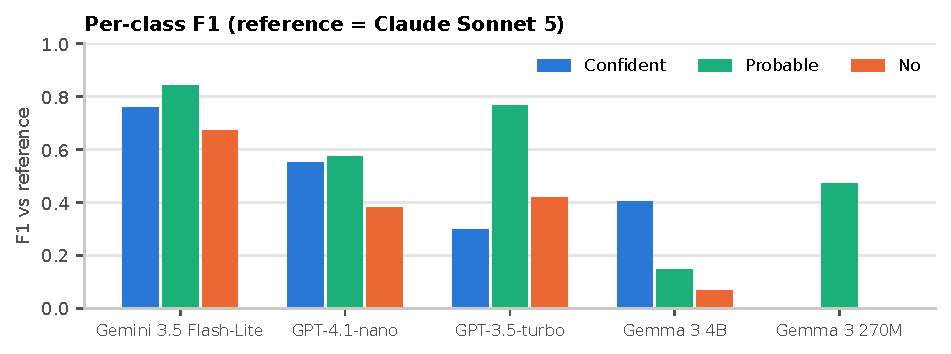
\includegraphics[width=0.85\linewidth]{figs/fig_perclass_f1.pdf}
\caption{Per-class F1 against the reference. Gemini 3.5 Flash-Lite is the only model above 0.65 on all three substantive classes. Gemma 3 4B predicts Confident far too often (recall 0.99, precision 0.25), whereas Gemma 3 270M never predicts it at all.}\label{fig:perclass}
\end{figure}

{\footnotesize
\begin{longtable}{>{\raggedright\arraybackslash}p{0.285\linewidth}>{\raggedright\arraybackslash}p{0.146\linewidth}>{\raggedright\arraybackslash}p{0.117\linewidth}>{\raggedright\arraybackslash}p{0.117\linewidth}>{\raggedright\arraybackslash}p{0.117\linewidth}>{\raggedright\arraybackslash}p{0.117\linewidth}}
\caption{Per-class precision, recall and F1 against the reference (shared pool, 73,845 abstracts). Reference support: Confident 17,206; Probable 43,929; No 7,805; No answer 4,905.}\label{tab:perclass}\\
\toprule
\textbf{Model} & \textbf{Class} & \textbf{Predicted} & \textbf{Precision} & \textbf{Recall} & \textbf{F1} \\
\midrule
\endfirsthead
\toprule
\textbf{Model} & \textbf{Class} & \textbf{Predicted} & \textbf{Precision} & \textbf{Recall} & \textbf{F1} \\
\midrule
\endhead
\bottomrule
\endlastfoot
Gemini 3.5 Flash-Lite & Confident & 16,160 & 0.785 & 0.737 & 0.760 \\
 & Probable & 50,665 & 0.787 & 0.908 & 0.843 \\
 & No & 6,573 & 0.735 & 0.619 & 0.672 \\
 & No answer & 447 & 0.266 & 0.024 & 0.044 \\
GPT-4.1-nano & Confident & 37,980 & 0.399 & 0.881 & 0.549 \\
 & Probable & 28,814 & 0.724 & 0.475 & 0.574 \\
 & No & 7,051 & 0.400 & 0.361 & 0.379 \\
 & No answer & 0 & --- & 0.000 & --- \\
GPT-3.5-turbo & Confident & 3,768 & 0.829 & 0.182 & 0.298 \\
 & Probable & 65,381 & 0.640 & 0.953 & 0.766 \\
 & No & 4,696 & 0.557 & 0.335 & 0.418 \\
 & No answer & 0 & --- & 0.000 & --- \\
Gemma 3 4B & Confident & 66,769 & 0.254 & 0.985 & 0.404 \\
 & Probable & 6,589 & 0.565 & 0.085 & 0.147 \\
 & No & 487 & 0.583 & 0.036 & 0.068 \\
 & No answer & 0 & --- & 0.000 & --- \\
Gemma 3 270M & Confident & 0 & --- & 0.000 & --- \\
 & Probable & 31,749 & 0.562 & 0.406 & 0.472 \\
 & No & 68 & 0.088 & 0.001 & 0.002 \\
 & No answer & 42,028 & 0.080 & 0.685 & 0.143 \\
\end{longtable}}

\begin{figure}[htbp]\centering
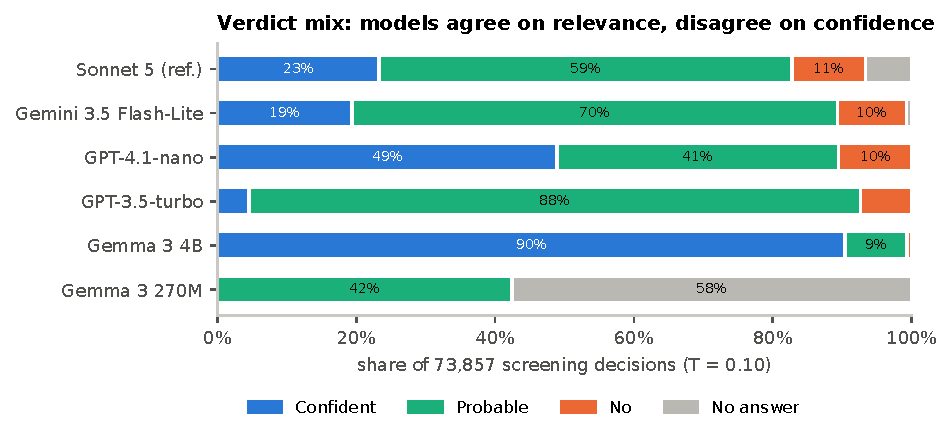
\includegraphics[width=0.85\linewidth]{figs/fig_verdict_mix.pdf}
\caption{Share of verdicts for each model across the full corpus at T = 0.10. For every model that parses reliably, the strict-or-yes accept rate sits between 83\% and 99\%, whereas the Confident share ranges from 0\% to 90\%, so the models largely agree on relevance and differ mainly in how confident they are.}\label{fig:verdicts}
\end{figure}

Table S4 looks separately at the accept/reject decision that each rule actually relies on. Under strict-only, the candidates' accept rates run from 0\% (Gemma 3 270M) to 90\% (Gemma 3 4B), compared with 23\% for the reference, which means the rule is measuring how willing each model is to commit just as much as it is measuring the literature.

\begin{table}[htbp]\centering\footnotesize
\caption{Binary accept/reject agreement at T = 0.10 under each acceptance rule. The reference accepts 23.3\% of abstracts under strict-only and 82.8\% under strict-or-yes.}\label{tab:binary}
\begin{tabular}{>{\raggedright\arraybackslash}p{0.295\linewidth}>{\raggedright\arraybackslash}p{0.170\linewidth}>{\raggedright\arraybackslash}p{0.170\linewidth}>{\raggedright\arraybackslash}p{0.151\linewidth}>{\raggedright\arraybackslash}p{0.122\linewidth}}
\toprule
\textbf{Model} & \textbf{Rule} & \textbf{Model accept rate} & \textbf{Raw agreement} & \textbf{Cohen's $\kappa$} \\
\midrule
Gemini 3.5 Flash-Lite & strict-only & 19.4\% & 89.0\% & 0.674 \\
 & strict-or-yes & 89.3\% & 88.6\% & 0.531 \\
GPT-4.1-nano & strict-only & 48.9\% & 67.9\% & 0.351 \\
 & strict-or-yes & 89.5\% & 82.0\% & 0.252 \\
GPT-3.5-turbo & strict-only & 4.5\% & 79.8\% & 0.214 \\
 & strict-or-yes & 92.7\% & 84.4\% & 0.289 \\
Gemma 3 4B & strict-only & 90.4\% & 32.2\% & 0.053 \\
 & strict-or-yes & 99.3\% & 83.0\% & 0.039 \\
Gemma 3 270M & strict-only & 0.0\% & 76.7\% & 0.000 \\
 & strict-or-yes & 42.3\% & 44.5\% & -0.009 \\
\bottomrule
\end{tabular}
\end{table}

Sampling temperature makes little difference. Each cloud model gives the same verdict at T = 0.10 and T = 0.15 for 93--97\% of abstracts ($\kappa$ = 0.85--0.89), and between the two temperatures the pair-level results in Tables S6--S7 shift by no more than 0.07 in $\rho$. The main analyses therefore use T = 0.10.

\begin{table}[htbp]\centering\footnotesize
\caption{Within-model stability across sampling temperature (T = 0.10 vs 0.15), abstract level.}\label{tab:temp}
\begin{tabular}{>{\raggedright\arraybackslash}p{0.371\linewidth}>{\raggedright\arraybackslash}p{0.168\linewidth}>{\raggedright\arraybackslash}p{0.214\linewidth}>{\raggedright\arraybackslash}p{0.168\linewidth}}
\toprule
\textbf{Model} & \textbf{Abstracts} & \textbf{Identical verdict} & \textbf{Cohen's $\kappa$} \\
\midrule
Gemini 3.5 Flash-Lite & 73,853 & 92.8\% & 0.846 \\
GPT-4.1-nano & 73,857 & 93.4\% & 0.887 \\
GPT-3.5-turbo & 73,857 & 96.8\% & 0.854 \\
\bottomrule
\end{tabular}
\end{table}

\section{S4  Pair-level agreement}
Tables S6 and S7 compare each system's pair priorities with the reference under the two rules. Rank agreement is Spearman's $\rho$ on the forecast SI level, and quadrant changes count the pairs that end up in a different quadrant. The $\pm$1 SD test counts pairs whose SI level falls within the reference's residual band, and the emerging columns compare which pairs land in the emerging quadrant, since that is the one most relevant to prioritising new research.

\begin{table}[htbp]\centering\footnotesize
\caption{Pair-level agreement with the reference under the \textbf{strict-only} rule (89 pairs). The reference places 13 pairs in the emerging quadrant (low level, rising shift).}\label{tab:pair_so}
\begin{tabular}{>{\raggedright\arraybackslash}p{0.303\linewidth}>{\raggedright\arraybackslash}p{0.093\linewidth}>{\raggedright\arraybackslash}p{0.110\linewidth}>{\raggedright\arraybackslash}p{0.084\linewidth}>{\raggedright\arraybackslash}p{0.093\linewidth}>{\raggedright\arraybackslash}p{0.102\linewidth}>{\raggedright\arraybackslash}p{0.102\linewidth}}
\toprule
\textbf{System} & \textbf{Spearman $\rho$} & \textbf{Quadrant changes} & \textbf{Top-5 overlap} & \textbf{Inside $\pm$1 SD} & \textbf{Emerging shared} & \textbf{Emerging Jaccard} \\
\midrule
Gemini 3.5 Flash-Lite (T=0.10) & 0.867 & 38\% & 4/5 & 70\% & 2/13 & 0.08 \\
Gemini 3.5 Flash-Lite (T=0.15) & 0.877 & 35\% & 4/5 & 73\% & 4/13 & 0.20 \\
GPT-4.1-nano (T=0.10) & 0.768 & 31\% & 3/5 & 54\% & 6/13 & 0.32 \\
GPT-4.1-nano (T=0.15) & 0.762 & 31\% & 3/5 & 53\% & 7/13 & 0.47 \\
GPT-3.5-turbo (T=0.10) & 0.620 & 45\% & 4/5 & 44\% & 3/13 & 0.16 \\
GPT-3.5-turbo (T=0.15) & 0.552 & 44\% & 3/5 & 42\% & 4/13 & 0.21 \\
Gemma 3 4B & 0.680 & 37\% & 3/5 & 52\% & 7/13 & 0.32 \\
Gemma 3 270M & --- & 72\% & 0/5 & 40\% & 0/13 & 0.00 \\
No LLM (accept all) & 0.665 & 39\% & 3/5 & 52\% & 6/13 & 0.26 \\
\bottomrule
\end{tabular}
\end{table}

\begin{table}[htbp]\centering\footnotesize
\caption{Pair-level agreement with the reference under the \textbf{strict-or-yes} rule (89 pairs). The reference places 11 pairs in the emerging quadrant.}\label{tab:pair_soy}
\begin{tabular}{>{\raggedright\arraybackslash}p{0.303\linewidth}>{\raggedright\arraybackslash}p{0.093\linewidth}>{\raggedright\arraybackslash}p{0.110\linewidth}>{\raggedright\arraybackslash}p{0.084\linewidth}>{\raggedright\arraybackslash}p{0.093\linewidth}>{\raggedright\arraybackslash}p{0.102\linewidth}>{\raggedright\arraybackslash}p{0.102\linewidth}}
\toprule
\textbf{System} & \textbf{Spearman $\rho$} & \textbf{Quadrant changes} & \textbf{Top-5 overlap} & \textbf{Inside $\pm$1 SD} & \textbf{Emerging shared} & \textbf{Emerging Jaccard} \\
\midrule
Gemini 3.5 Flash-Lite (T=0.10) & 0.967 & 10\% & 4/5 & 94\% & 9/11 & 0.60 \\
Gemini 3.5 Flash-Lite (T=0.15) & 0.962 & 15\% & 4/5 & 90\% & 8/11 & 0.44 \\
GPT-4.1-nano (T=0.10) & 0.924 & 21\% & 4/5 & 88\% & 8/11 & 0.38 \\
GPT-4.1-nano (T=0.15) & 0.927 & 21\% & 4/5 & 87\% & 7/11 & 0.35 \\
GPT-3.5-turbo (T=0.10) & 0.923 & 17\% & 4/5 & 89\% & 8/11 & 0.47 \\
GPT-3.5-turbo (T=0.15) & 0.932 & 17\% & 4/5 & 92\% & 8/11 & 0.47 \\
Gemma 3 4B & 0.951 & 16\% & 4/5 & 89\% & 9/11 & 0.50 \\
Gemma 3 270M & 0.831 & 34\% & 2/5 & 53\% & 6/11 & 0.33 \\
No LLM (accept all) & 0.951 & 13\% & 4/5 & 90\% & 9/11 & 0.50 \\
\bottomrule
\end{tabular}
\end{table}

\begin{figure}[htbp]\centering
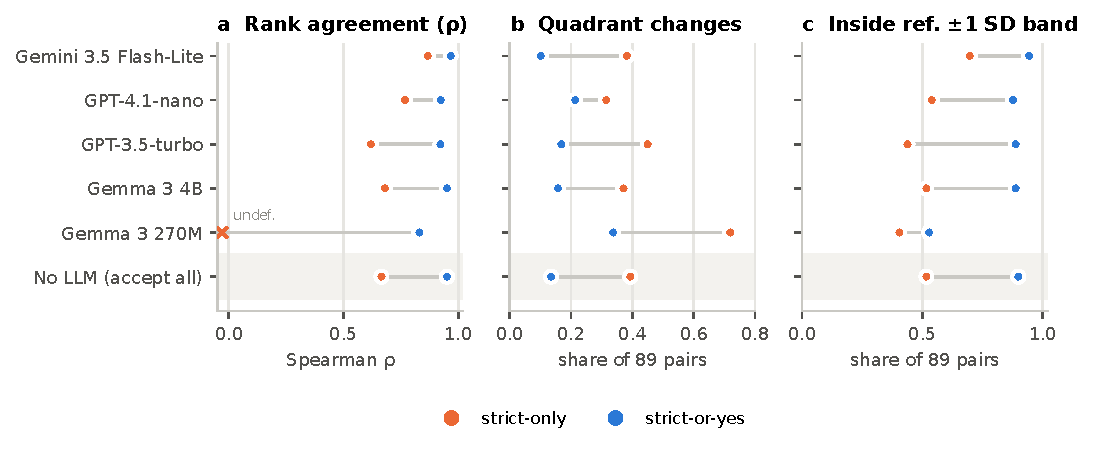
\includegraphics[width=1.00\linewidth]{figs/fig_rule_effect.pdf}
\caption{The same models under the two acceptance rules. Every system improves on every pair-level measure when the rule is relaxed. The shaded row is the no-LLM baseline, which accepts every retrieved abstract.}\label{fig:rule}
\end{figure}

\begin{figure}[htbp]\centering
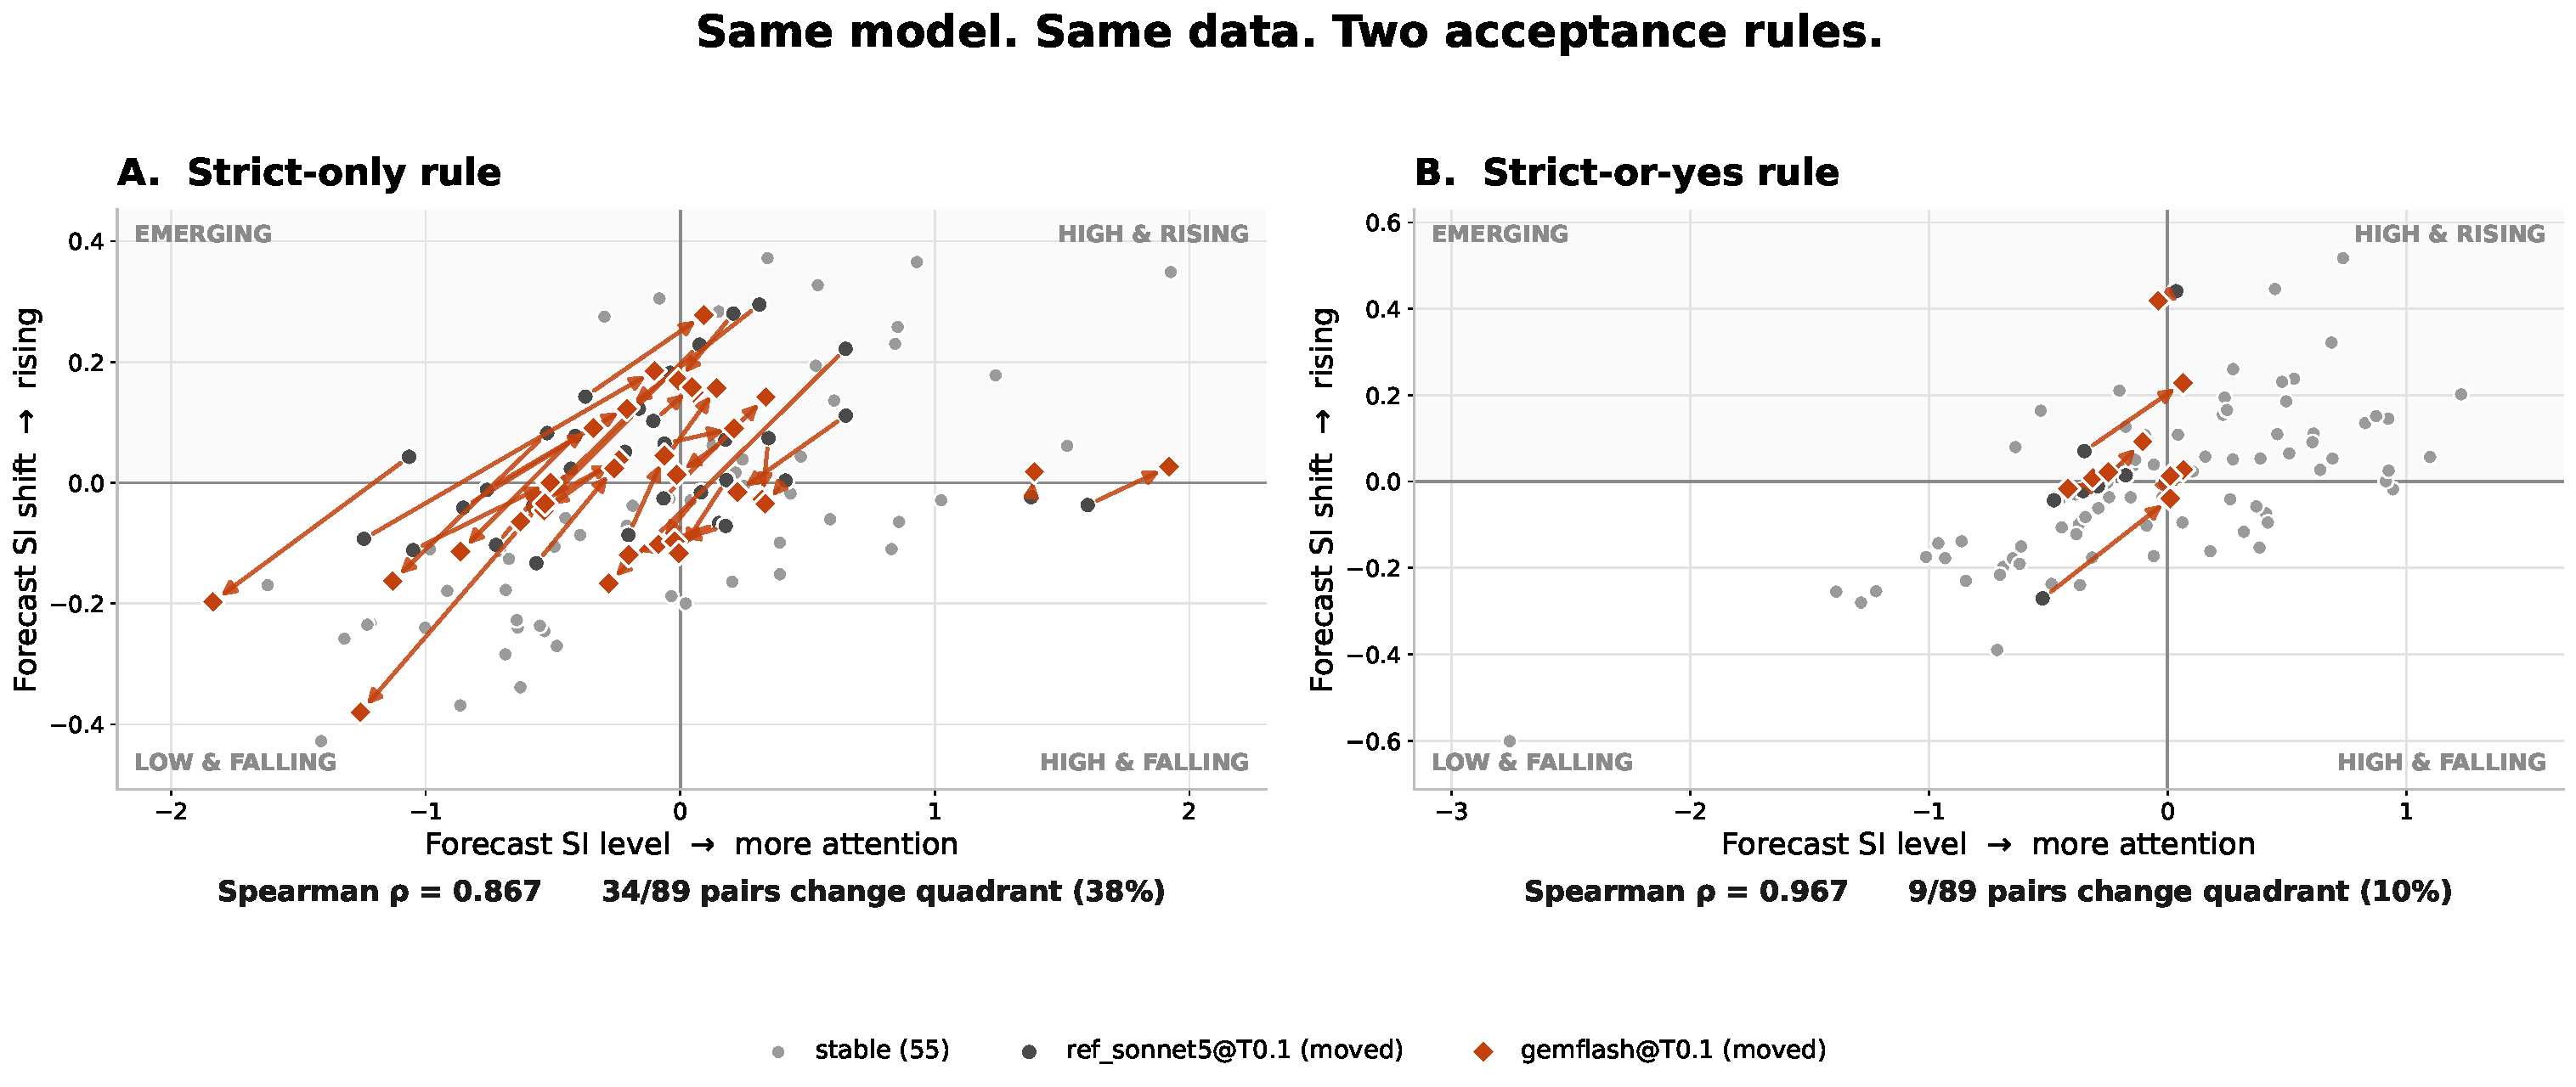
\includegraphics[width=1.00\linewidth]{figs/fig_quadrant_hero.pdf}
\caption{Priority map for Gemini 3.5 Flash-Lite against the reference. Wherever a pair changes quadrant, an arrow runs from its reference position to its Gemini position; this happens for 34 of 89 pairs under strict-only and 9 of 89 under strict-or-yes.}\label{fig:hero}
\end{figure}

\subsection{S4.1  The rule interacts with the model rather than simply shifting results}
If the acceptance rule just moved every model by the same amount, the candidates would disagree with one another to the same extent under both rules, and they do not. As Table S8 shows, two candidates place 22--52\% of pairs in different quadrants under strict-only (43--52\% among the three API models), but only 11--16\% under strict-or-yes. With a permissive rule the choice of model hardly matters, whereas with a strict one it largely determines the result.

\begin{figure}[htbp]\centering
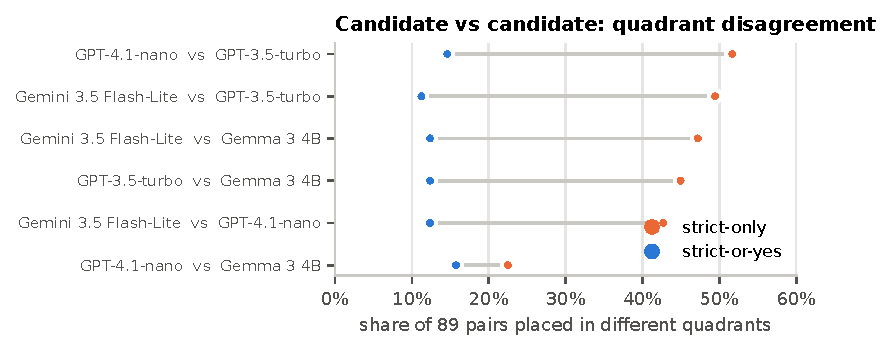
\includegraphics[width=0.75\linewidth]{figs/fig_model_vs_model.pdf}
\caption{Quadrant disagreement between every pair of full-coverage candidate models.}\label{fig:mvm}
\end{figure}

\begin{table}[htbp]\centering\footnotesize
\caption{Candidate-versus-candidate disagreement: share of the 89 pairs that two candidate models place in different priority quadrants (T = 0.10).}\label{tab:mvm}
\begin{tabular}{>{\raggedright\arraybackslash}p{0.304\linewidth}>{\raggedright\arraybackslash}p{0.304\linewidth}>{\raggedright\arraybackslash}p{0.157\linewidth}>{\raggedright\arraybackslash}p{0.157\linewidth}}
\toprule
\textbf{Model A} & \textbf{Model B} & \textbf{strict-only} & \textbf{strict-or-yes} \\
\midrule
Gemini 3.5 Flash-Lite & GPT-4.1-nano & 43\% & 12\% \\
Gemini 3.5 Flash-Lite & GPT-3.5-turbo & 49\% & 11\% \\
Gemini 3.5 Flash-Lite & Gemma 3 4B & 47\% & 12\% \\
GPT-4.1-nano & GPT-3.5-turbo & 52\% & 15\% \\
GPT-4.1-nano & Gemma 3 4B & 22\% & 16\% \\
GPT-3.5-turbo & Gemma 3 4B & 45\% & 12\% \\
\bottomrule
\end{tabular}
\end{table}

\subsection{S4.2  No-LLM baseline}
The baseline counts every retrieved co-mention abstract as accepted and then runs exactly the same SI build. Under strict-or-yes it agrees with the reference at $\rho$ = 0.951, with 13.5\% of pairs changing quadrant and 9 of the 11 emerging pairs shared. That puts it level with Gemma 3 4B and ahead of GPT-4.1-nano, GPT-3.5-turbo and Gemma 3 270M. This happens because the reference itself accepts 82.8\% of abstracts under strict-or-yes, so its accepted counts closely follow the raw co-mention counts. The high strict-or-yes agreement in earlier drafts is therefore better understood as agreement about publication volume than as evidence that the models judge relevance in the same way. Under strict-only the baseline drops to $\rho$ = 0.665, with 39\% of pairs changing quadrant. Here Gemini 3.5 Flash-Lite ($\rho$ = 0.867) and GPT-4.1-nano ($\rho$ = 0.768) clearly improve on it, while GPT-3.5-turbo (0.620) and Gemma 3 4B (0.680) do not.

\subsection{S4.3  Per-paper and aggregate agreement measure different things}
Gemma 3 270M has $\kappa$ = $-$0.009 against the reference, yet under strict-or-yes it ranks pairs at $\rho$ = 0.831, which is higher than GPT-3.5-turbo manages under strict-only (0.620). Adding up thousands of noisy verdicts for each pair smooths out much of the label noise, and a pooled regression on counts rewards getting the volume right more than getting individual abstracts right. Had we relied on a headline correlation, we would have recommended a model that agrees with the reference on almost no individual paper. Under strict-only, the same model produces no Confident verdicts at all, so its SI signal is constant and $\rho$ cannot be calculated.

\section{S5  Model size ladder}
To find where screening breaks down, we ran six small open-weight configurations on three representative pairs chosen with the supervisors (5,051 abstracts). The breakdown is not gradual. Gemma 3 270M gives a parseable verdict for only 42\% of abstracts, and even then it never answers Confident. Gemma 3 4B parses every abstract but calls 93--95\% of them Confident, so its failure is over-commitment rather than formatting. Qwen 3 parses every abstract even at 0.6B, which suggests that the formatting threshold depends on the model family and its training, not just on parameter count. The Gemma 3 1B run stalled after 22 screens, so we do not interpret it, and an earlier draft figure that showed it without a coverage guard has been withdrawn.

\begin{figure}[htbp]\centering
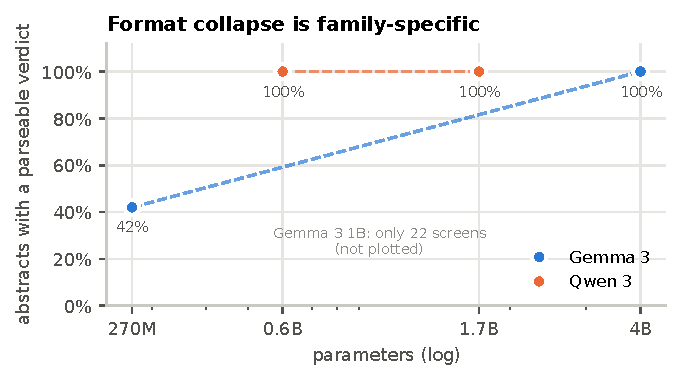
\includegraphics[width=0.60\linewidth]{figs/fig_size_ladder.pdf}
\caption{Share of abstracts with a parseable verdict on the three-pair slice.}\label{fig:ladder}
\end{figure}

\begin{table}[htbp]\centering\footnotesize
\caption{Size ladder on the three shared pairs (\emph{K. pneumoniae}--ciprofloxacin, \emph{A. baumannii}--tigecycline, \emph{E. coli}--ceftazidime; 5,051 abstracts), T = 0.10. Parseable = any verdict other than No answer.}\label{tab:ladder}
\begin{tabular}{>{\raggedright\arraybackslash}p{0.178\linewidth}>{\raggedright\arraybackslash}p{0.118\linewidth}>{\raggedright\arraybackslash}p{0.078\linewidth}>{\raggedright\arraybackslash}p{0.138\linewidth}>{\raggedright\arraybackslash}p{0.108\linewidth}>{\raggedright\arraybackslash}p{0.118\linewidth}>{\raggedright\arraybackslash}p{0.148\linewidth}}
\toprule
\textbf{Model} & \textbf{Family} & \textbf{Params} & \textbf{Route} & \textbf{Screens} & \textbf{Parseable} & \textbf{Confident share} \\
\midrule
gemma3\_270m & Gemma 3 & 270M & local & 5,051 & 42\% & 0\% \\
gemma3\_1b & Gemma 3 & 1B & local & 22 (partial) & 95\% & 23\% \\
gemma3\_4b & Gemma 3 & 4B & local & 5,051 & 100\% & 95\% \\
gemma3\_4b\_or & Gemma 3 & 4B & OpenRouter & 5,051 & 100\% & 93\% \\
qwen3\_06b & Qwen 3 & 0.6B & local & 5,051 & 100\% & 26\% \\
qwen3\_17b & Qwen 3 & 1.7B & local & 3,480 (partial) & 100\% & 66\% \\
\bottomrule
\end{tabular}
\end{table}

\section{S6  Cost analysis}
\subsection{S6.1  Method}
The cost per paper is the API cost of a single screening call, that is, input tokens $\times$ input price plus output tokens $\times$ output price. To measure input length, we rebuilt the exact prompt for all 73,849 reference screens (system message, instruction, title and abstract), converted characters to tokens at four characters per token, and added 12 tokens for the chat template. This gives a mean of 848 tokens (median 848, 95th percentile 1,094). Output length was measured for each model from the stored raw replies and comes to 12--19 tokens. Claude Sonnet 5 uses adaptive thinking, which is billed as output but does not appear in the stored text, so to be conservative we billed its output at the 60-token cap. Prices are the list prices recorded in the pipeline configuration at the time of each run (Table S10). Local inference appears as \$0 in API fees, but it is not free: Gemma 3 270M took about 84 hours of wall-clock time on a single RTX 4080.

\begin{table}[htbp]\centering\footnotesize
\caption{Screening cost per paper and per corpus at list prices (USD per million tokens, input/output, as recorded in the pipeline configuration, July--August 2026). Input $\approx$ 848 tokens per call (prompt + title + abstract, measured); output measured per model. Sonnet 5 is priced at the Batch API rate (50\% off list) with output billed at the 60-token cap; its standard-API cost is \$3.45 per 1,000 papers. Full corpus = 73,849 paper--pair screens.}\label{tab:cost}
\begin{tabular}{>{\raggedright\arraybackslash}p{0.212\linewidth}>{\raggedright\arraybackslash}p{0.100\linewidth}>{\raggedright\arraybackslash}p{0.084\linewidth}>{\raggedright\arraybackslash}p{0.092\linewidth}>{\raggedright\arraybackslash}p{0.084\linewidth}>{\raggedright\arraybackslash}p{0.076\linewidth}>{\raggedright\arraybackslash}p{0.052\linewidth}>{\raggedright\arraybackslash}p{0.076\linewidth}>{\raggedright\arraybackslash}p{0.084\linewidth}}
\toprule
\textbf{Model} & \textbf{Price in / out} & \textbf{Per paper} & \textbf{Per 1,000 papers} & \textbf{Full corpus} & \textbf{vs reference} & \textbf{$\kappa$} & \textbf{$\rho$ strict-only} & \textbf{$\rho$ strict-or-yes} \\
\midrule
Claude Sonnet 5 (reference) & 3.00 / 15.00 & \$0.0017 & \$1.72 & \$127.22 & 100.0\% & 1 & 1 & 1 \\
Gemini 3.5 Flash-Lite & 0.30 / 2.50 & \$0.00028 & \$0.28 & \$20.97 & 16.5\% & 0.58 & 0.87 & 0.97 \\
GPT-4.1-nano & 0.10 / 0.40 & \$0.00009 & \$0.09 & \$6.62 & 5.2\% & 0.26 & 0.77 & 0.92 \\
GPT-3.5-turbo & 0.50 / 1.50 & \$0.00044 & \$0.44 & \$32.74 & 25.7\% & 0.22 & 0.62 & 0.92 \\
Gemma 3 4B & 0.05 / 0.10 & \$0.000044 & \$0.04 & \$3.23 & 2.5\% & 0.03 & 0.68 & 0.95 \\
Gemma 3 270M & 0.00 / 0.00 & \$0 & \$0.00 & \$0.00 & 0.0\% & -0.01 & --- & 0.83 \\
No LLM (accept all) & --- & \$0.00 & \$0.00 & \$0.00 & 0\% & --- & 0.67 & 0.95 \\
\bottomrule
\end{tabular}
\end{table}

\begin{figure}[htbp]\centering
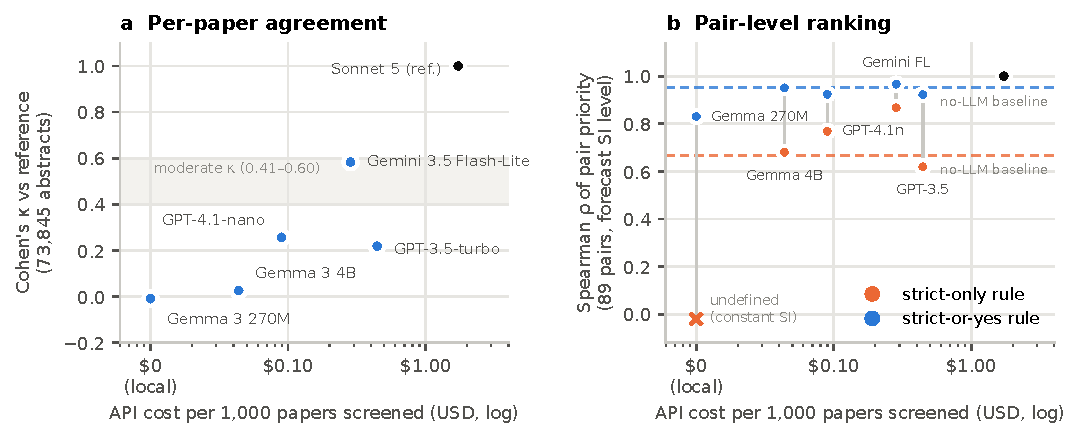
\includegraphics[width=1.00\linewidth]{figs/fig_cost_performance.pdf}
\caption{Cost against fidelity. (a) Abstract-level $\kappa$ plotted against API cost per 1,000 papers. (b) Pair-level rank agreement under each acceptance rule, with dashed lines marking the no-LLM baseline for each rule. Under strict-or-yes nearly every model sits at or below the free baseline. Under strict-only, spending more does buy agreement, but only Gemini 3.5 Flash-Lite buys much of it.}\label{fig:cost}
\end{figure}

\subsection{S6.2  Reading the curve}
Gemini 3.5 Flash-Lite is the only model on the efficient frontier that beats the no-LLM baseline under both rules. It costs 16\% of the reference, which would cut the full corpus from \$127 to \$21. GPT-4.1-nano is the cheapest model that clearly beats the baseline under strict-only, at 5\% of the reference cost, although its per-paper agreement is only fair. GPT-3.5-turbo is dominated, since it costs more than Gemini 3.5 Flash-Lite and does worse on every measure. For anyone who only needs the strict-or-yes ranking, the results suggest the language model could be left out altogether.

\subsection{S6.3  Sensitivity}
Four characters per token is a standard approximation, and tokenisers differ by roughly $\pm$15\% on biomedical text. That would change every cost by the same proportion without changing the ranking. If Sonnet 5 is billed at its measured visible output of about 12 tokens rather than the 60-token cap, the reference drops to \$1.36 per 1,000 papers, and running it on the standard API instead of the Batch API doubles the cost to \$3.45. Adding up the configurations we actually ran (the reference once, three cloud models at two temperatures and Gemma 3 4B once) gives an estimated screening spend of \$251. This fits with the budget of about \$285 approved in July 2026, which also covered the halted Gemini 3 Flash Preview run.

\section{S7  Limitations and threats to validity}
\begin{itemize}
\item \textbf{No human ground truth.} Agreement is measured against Claude Sonnet 5 rather than expert annotators, so the study shows how far cheaper models drift from a strong model, not how often any of them is actually right. A stratified sample of a few hundred human-labelled abstracts would give every number here a firm anchor.
\item \textbf{Empty reference completions.} Of the reference screens, 4,905 (6.6\%) are No answer, and 4,807 of those are completely empty. The most likely explanation is that adaptive thinking used up the 60-token output cap before any JSON was written. These abstracts are treated as a class in $\kappa$ and left out of the accepted counts under both rules, so they pull every model's $\kappa$ down slightly. They should be re-run with a larger output budget before submission.
\item \textbf{Mixed reference routing.} 789 reference screens (1.1\%) went through OpenRouter instead of the Batch API. The model is the same, but the provider's default settings may not be.
\item \textbf{One prompt.} Every result depends on a single fixed prompt and verdict scale, and we did not test how sensitive the results are to the prompt.
\item \textbf{Size ladder coverage.} The ladder covers only 3 of the 89 pairs, the Gemma 3 1B rung is missing and the Qwen 3 1.7B rung is 69\% complete. The local LM Studio weights are quantised, so local and hosted results for the same model are reported separately.
\item \textbf{Pooled regression.} Because the pathogen and antibiotic coefficients are fitted jointly, reclassifying one pair can shift the SI of other pairs that share its pathogen or antibiotic, so pair-level disagreements are not independent of one another.
\item \textbf{Skewed pair sizes.} Pairs with very few abstracts (the smallest has just 2) have unstable SI trajectories and can change quadrant because of a handful of verdicts.
\item \textbf{Prices change.} The costs use list prices recorded in July--August 2026, so the relative costs are likely to hold up better than the absolute ones.
\end{itemize}
\section{S8  Reproducibility}
Every number in this supplement can be regenerated from the project database (\texttt{output/amr.sqlite}, 366 MB) with three scripts and no manual steps:

\begin{itemize}
\item \texttt{build\_si.py} builds SI trajectories, forecasts and quadrant tables for both rules (default settings, Table S11).
\item \texttt{analyse\_all.py} recomputes abstract-level, pair-level, size-ladder and cost results into CSV files and \texttt{facts.json}.
\item \texttt{make\_pub\_figures.py} draws every figure in this supplement from those CSV files.
\item The no-LLM baseline is added by inserting one accept-all verdict for each reference screen into a copy of the database, before running \texttt{build\_si.py}.
\end{itemize}
\begin{table}[htbp]\centering\footnotesize
\caption{Analysis settings used for every number in this supplement.}\label{tab:settings}
\begin{tabular}{>{\raggedright\arraybackslash}p{0.404\linewidth}>{\raggedright\arraybackslash}p{0.542\linewidth}}
\toprule
\textbf{Setting} & \textbf{Value} \\
\midrule
SI year window & 2000--2025 (partial 2026 excluded) \\
Shared abstract pool & 70,360 abstracts judged by all nine full-coverage systems \\
Regression & Pooled ridge, $\alpha$ = 1.0; log accepted count \textasciitilde{} log background counts + pathogen + antibiotic one-hots \\
Smoothing & LOWESS, frac = 0.5 \\
Forecast & Damped slope, horizon 5 years, slope window 6 years, damping half-life 3 years \\
Quadrants & Split at 0 on forecast SI level and forecast SI shift \\
Band test & Candidate SI level inside reference level $\pm$ 1 residual SD \\
Coverage guard & Systems below 50\% of reference screens excluded \\
Reference & Claude Sonnet 5, single pass; custom temperature rejected by the model \\
\bottomrule
\end{tabular}
\end{table}

\section{S9  Engineering notes worth keeping}
Several problems we found while building the pipeline would have silently corrupted a result like this one, and each now has a guard:

\begin{itemize}
\item \textbf{Duplicate abstracts across years.} We found and removed 6,955 duplicate pair--abstract rows before screening, and \texttt{DISTINCT} now protects both the screening queue and the export.
\item \textbf{Batch placeholders.} Batch items that errored used to be saved as permanent uncertain rows, which stopped them from ever being retried. Temporary errors are now left pending and retried, and only permanent failures are stored.
\item \textbf{Temperature deprecation.} Sonnet 5 rejects a custom temperature, so the adapters now detect this and retry without it instead of failing.
\item \textbf{Coverage guards.} A partial run of 22 rows was once plotted as though it were complete. All analysis scripts now drop systems below 50\% coverage and state the exclusion on the figure.
\item \textbf{Fair macro-F1.} The original macro-F1 penalised Gemini 3.5 Flash-Lite for being the only model that ever outputs No answer (0.580 against 0.758). The reported figure averages over the three substantive classes instead.
\item \textbf{Resumable pipeline.} Every stage saves its progress to SQLite, can be interrupted safely and picks up again without re-fetching or re-screening, which is what made a 700,000-call study possible on a laptop.
\end{itemize}
\end{document}